\chapter{Introduction}\label{chapter:introduction}
Modern computer systems are facing TODO. Users are one of the most commonly exploited things around computers, especially in social engineering and fishing. Most systems currently rely on a standard combination between username and password. Already in 2009, Aloul et al.\ described the most common security concerns with passwords:\cite{aloul2009two}
``Users tend to use easy-to-guess passwords, use the same password in multiple accounts, write the passwords or store them on their machines, etc. Furthermore, hackers have the option of using many techniques to steal passwords such as shoulder surfing, snooping, sniffing, guessing, etc.''

Furthermore, many users tend to stay logged into services with their mobile devices, despite not having appropriate security measures for their devices. On most Android phones, full disk encryption is not enabled by default, which leads to another attack vector for identity theft.

Aloul et al.\ introduced a system of \glspl{otp} using mobile phones, which significantly improves security by introducing a second factor of authentication. However, for authentication situations on smartphones themselves the \gls{otp} mechanism is rendered pretty much useless, as the second factor is in fact on the same device.

\cite{bishop2006pattern}
\section{Vision}
The whole vision of this thesis, is to provide a way to easily detect individual users by a short authentication sequence based on acceleration patterns. Even though this does not qualify as cryptographically secure authentication, behavioural patterns and keystroke recognition can be used as biometric authentication aids. For example, Bhargav-Spantzel et. al.\cite{bhargav2006privacy}\ described a system to extract cryptographic biometric keys from biometric data and how this can be combined with additional other proofs of identity to provide strong authentication.

With acceleration pattern recognition, we will make a authentication mechanism with zero additional user interaction possible. This allows for higher frequency user re-authentication without disturbing and annoying the user. That means, instead of prompting the user with a login screen every 24 hours, we can measure his or her acceleration patterns every time sensitive information is accessed. Therefore, we can not only provide basic login authentication, but also provide a way for users to stay authenticated for longer sessions or even detect when someone else hijacks a valid session. Since the time between two authentication requests can almost be arbitrarily small, an attacker who gets control over the current session will get a new authentication request relatively quickly, thus minimizing the potential damage.
\section{Single user licenses}
Another application of this technique is to identify individual users, even if using the same device. This might not only be useful in terms of individualizing the software according to the current user, but also for tracking of software usage.

A common licensing model for software are per-user licenses, i.e.\ $n$ licenses for $n$ users of the software. However, this license model currently cannot be enforced, since the software is installed on a single physical device, which may be shared among users. This led to most software companies licensing their software per-installation instead of per-user.
As of 2016, many users tend to have multiple devices and also want to use their licenses on multiple devices. This resulted in a trend to bind software licenses to user accounts instead of devices. This trend is also prevailing in modern \gls{saas} models, which do not require installation of the software on end-user devices anymore.
A possible circumvention of these account bound licenses is account sharing. This imposes a real problem, not only for software licensors, but also for other access providers. For example a consumer research from Parks Associates\cite{accountsharing} reports, that ``6\% [of video streaming users] are exclusively using shared accounts to access subscription''. 

The methods described in this theses can give a powerful way to detect individual users sharing physical devices, as well as sharing individual accounts and thus reduce copyright infringements that could not even be detected beforehand.

\section{Multi-factor authentication}
\gls{mfa} is a technique to enhance security in access control situations. It combines multiple forms of authentication mechanisms, based on conceptually different approaches: Knowledge, e.g.\ passwords or PINs; possessions, e.g.\ keys or bank cards and biometric characteristics, like fingerprints or, as in our approach, behavioural patterns.

A typical authentication attempt with \gls{mfa} is only successful, when all needed factors are present. The most common example for \gls{mfa} is banking, where one needs to be in possession of the banking card and needs to know the card's PIN. However, an attack vector targeting this system is copying the banking card while the attacked person does not notice his card being copied. This attack vector is also possible with biometric characteristics and even relatively easy, as many biometric traits are publicly visible. Fingerprints have proven to be copyable with low cost\cite{starbug2008bastel} and new high resolution cameras allow to photograph fingerprints and eyes in high enough quality to spoof many scanners\cite{fiebig2014security}. These attacks also can be adapted to other authentication systems based on visible biometric traits, such as iris recognition or Android's Face Unlock.

For biometric authentication to be sufficiently secure, the traits need to be intrinsic, i.e.\ not publicly visible, and hard to copy. Acceleration based motion detection matches these requirements, as recording of these patterns is only possible with physical access to the authentication device or very close monitoring of all body movement of the user.

\section{Smart mobile devices}
Smart devices are electronic devices, that feature wireless communication, e.g.\ WiFi or Bluetooth. Smart \emph{mobile} devices are smart devices, that are typically worn or kept in close proximity to the user. This usage usually results in small form factors and little weight. These devices are most often commodity devices and used frequently. Therefore, smart mobile devices are ideal to provide authentication, since the authenticating user is accustomed using the device.

\begin{figure}
    \centering
    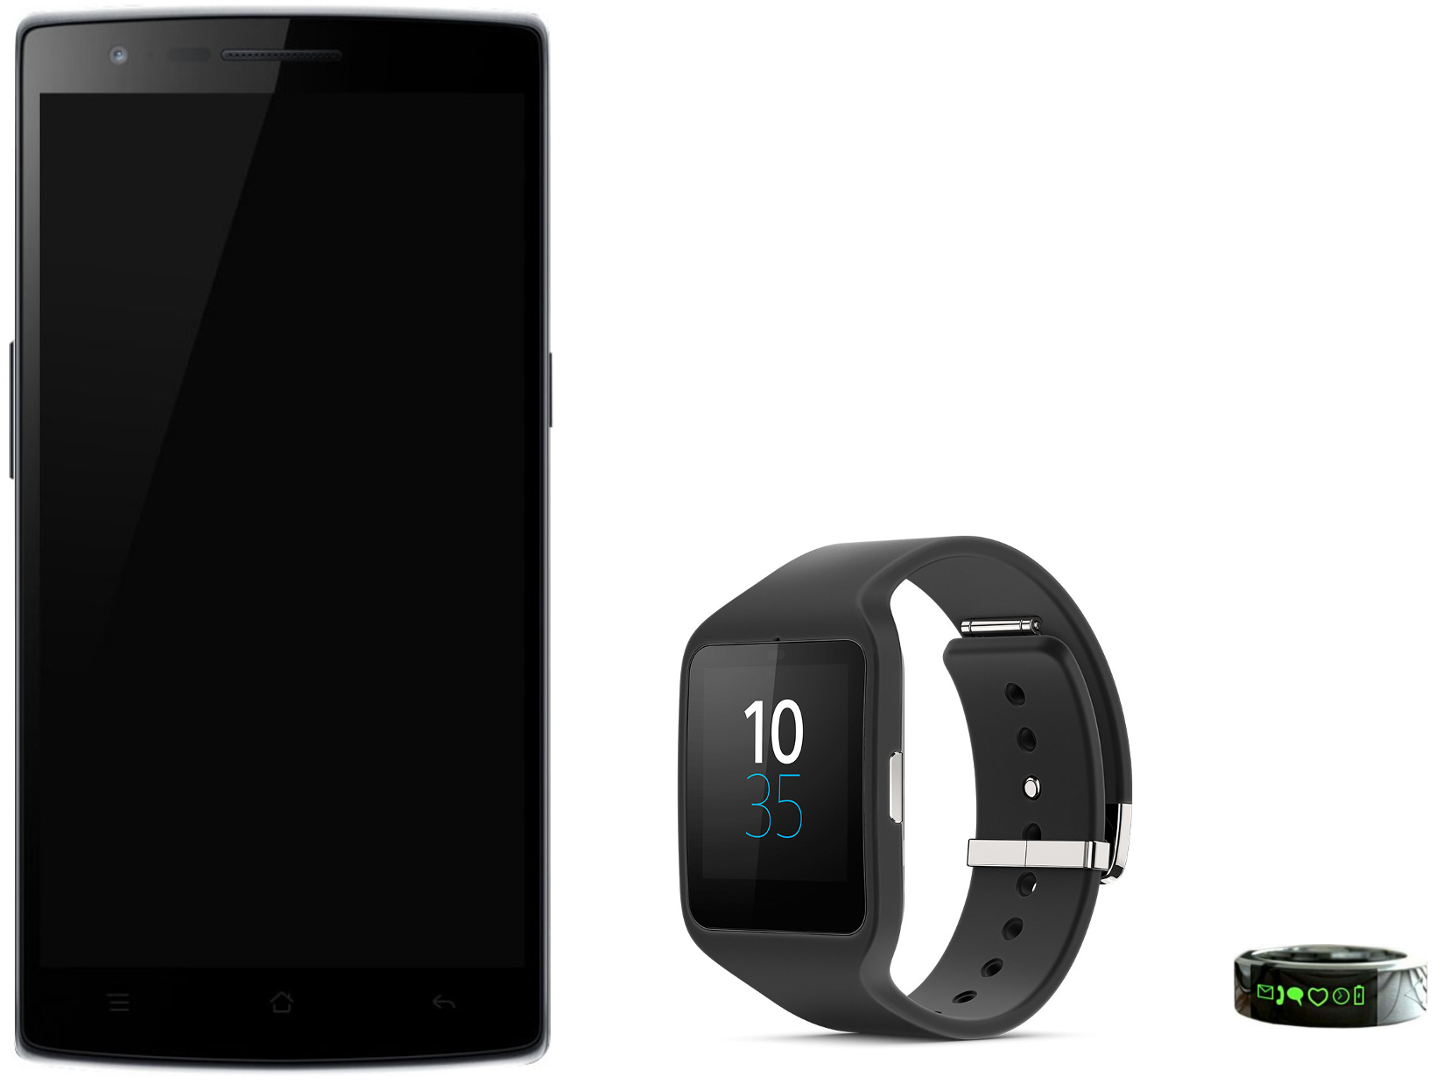
\includegraphics[width=\textwidth]{figures/SmartDevices.png}
    \caption{Examples for smart mobile devices that are worn in close proximity of the user (from left to right): A OnePlus One smartphone, a Sony SmartWatch 3, Smarty Ring concept design}
    \label{fig:smartdevices}
\end{figure}
Common examples for smart mobile devices are smartphones and smartwatches.
TODO: Füllbild beschreiben

\subsection{Smartphones}
Smartphones are the most capable of the smart mobile devices discussed herein. Smartphones usually have numerous wireless communication possibilities and thus function are a personal data-hub, to which other personal devices connect and communicate over. Typical connections for Smartphones are: Cellular network (e.g.\ \acrshort{gsm}, \acrshort{umts}), WiFi, Bluetooth, Near Field Communication etc. Smartphones are also packed with sensors, which can be utilized by programmers of \Glspl{app} and typically include acceleration as well as gyroscopic sensors for movement detection.

TODO: Android, IOS, WindowsPhone -> Android biggest target audience
\subsection{Smartwatches}
Smartwatches, bild mitte, beginn von Android Wear, adaption smartphone/smartwatch -> alles android

TODO: Operating systems: more differenciated. Android, WatchOS, Tizen, PebbleOS Market share from \cite{idc2015wristmarketshare}

\subsection{Smart-rings}
Future music, no real sensors, maybe special developement necessary to identify users with accelerometers?

\section{Pattern recognition}
TODO: hier schaubild einfügen
\subsection{Preprocessing}
\subsection{Feature extraction}
Dynamic time warping
\subsection{Classification}
Support Vector Machine
TODO Schaubild für SVM

k-Nearest Neighbor
TODO Schaubild für KNN

Bayes classifier

Neuronal networks

Machine learning with encog

Tensorflow